\section{Logic, Shift and Rotate Instructions}

\begin{concept}{Logic Instructions}\\
Base logic operations (affect only N and Z flags):
\begin{itemize}
  \item \textbf{ANDS}: Bitwise AND (Rdn \& Rm, a \& b)
  \item \textbf{BICS}: Bit Clear (Rdn \& !Rm, a \& ~b)
  \item \textbf{EORS}: Exclusive OR (Rdn \textdollar Rm, a $\wedge$  b)
  \item \textbf{MVNS}: Bitwise NOT (!Rm, ~a)
  \item \textbf{ORRS}: Bitwise OR (Rdn \# Rm, a | b)
\end{itemize}
\end{concept}

\begin{concept}{Shift and Rotate Instructions}\\
Shift operations for binary manipulation:
\begin{itemize}
  \item \textbf{LSLS}: Logical Shift Left ($2^n \cdot Rn$, 0 → LSB)
  \item \textbf{LSRS}: Logical Shift Right ($2^{-n} \cdot Rn$, 0 → MSB)
  \item \textbf{ASRS}: Arithmetic Shift Right ($R^{-n}$, ±MSB → MSB)
  \item \textbf{RORS}: Rotate Right (LSB → MSB)
\end{itemize}

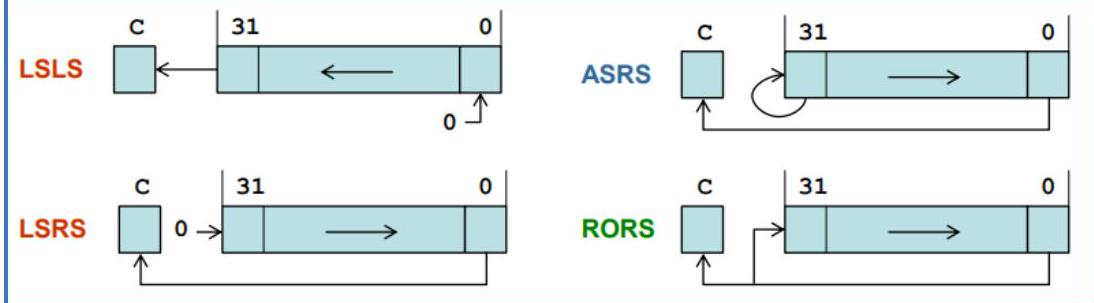
\includegraphics[width=\linewidth]{images/2024_12_29_79e6b22f503fb7b4f718g-06}
\end{concept}

\begin{definition}{Integer Casting}\\
\textbf{Extension (adding bits):}
\begin{itemize}
  \item \textbf{Zero Extension} (unsigned):
    \begin{itemize}
      \item Fill left bits with zero
      \item Example: 1011 → 00001011
    \end{itemize}
  \item \textbf{Sign Extension} (signed):
    \begin{itemize}
      \item Copy sign bit to the left
      \item Example: 1011 → 11111011
    \end{itemize}
\end{itemize}

\textbf{Truncation (removing bits):}
\begin{itemize}
  \item Signed: May change sign
  \item Unsigned: Results in modulo operation
\end{itemize}
\end{definition}

\begin{example2}{Integer Ranges by Word Size}
\textbf{8-bit integers:}
\begin{itemize}
  \item Unsigned: 0 to 255 (0x00 to 0xFF)
  \item Signed: -128 to 127 (0x80 to 0x7F)
\end{itemize}

\textbf{16-bit integers:}
\begin{itemize}
  \item Unsigned: 0 to 65,535 (0x0000 to 0xFFFF)
  \item Signed: -32,768 to 32,767 (0x8000 to 0x7FFF)
\end{itemize}

\textbf{32-bit integers:}
\begin{itemize}
  \item Unsigned: 0 to 4,294,967,295 (0x00000000 to 0xFFFFFFFF)
  \item Signed: -2,147,483,648 to 2,147,483,647 (0x80000000 to 0x7FFFFFFF)
\end{itemize}
\end{example2}

\begin{example2}{Logical Operations}
Common logic operations:
\begin{lstlisting}[language=armasm, style=basesmol]
    ; Logic operations
    ANDS R0, R1         ; R0 = R0 AND R1
    BICS R0, R1         ; R0 = R0 AND NOT R1
    EORS R0, R1         ; R0 = R0 XOR R1
    MVNS R0, R1         ; R0 = NOT R1
    ORRS R0, R1         ; R0 = R0 OR R1
    
    ; Shift operations
    LSLS R0, R1, #2     ; R0 = R1 << 2 (multiply by 4)
    LSRS R0, R1, #1     ; R0 = R1 >> 1 (divide by 2)
    ASRS R0, R1, #2     ; R0 = R1 >> 2 (signed divide by 4)
    RORS R0, R1, #1     ; Rotate R1 right by 1 bit
\end{lstlisting}
\end{example2}

\begin{KR}{Using Logic and Shift Instructions}\\
Steps for bit manipulation:
\begin{enumerate}
  \item Identify required operation (AND, OR, XOR, NOT, shift)
  \item Choose appropriate instruction
  \item Consider effect on flags if relevant
  \item For shifts:
    \begin{itemize}
      \item LSLS for multiplication by $2^n$
      \item LSRS for unsigned division by $2^n$
      \item ASRS for signed division by $2^n$
    \end{itemize}
  \item For logic:
    \begin{itemize}
      \item ANDS for bit masking
      \item ORRS for bit setting
      \item BICS for bit clearing
      \item EORS for bit toggling
    \end{itemize}
\end{enumerate}
\end{KR}

\begin{concept}{Flag Behavior with Logic Instructions}\\
Logic instructions only affect N and Z flags:
\begin{itemize}
  \item \textbf{N flag}: Set to bit 31 of result (MSB)
  \item \textbf{Z flag}: Set if result is zero
  \item \textbf{C flag}: Unchanged
  \item \textbf{V flag}: Unchanged
\end{itemize}

Special case for shift/rotate:
\begin{itemize}
  \item \textbf{C flag}: Set to last bit shifted out
  \item \textbf{N,Z flags}: Set based on result
  \item \textbf{V flag}: Unchanged
\end{itemize}
\end{concept}

\begin{KR}{Bit Manipulation Techniques}\\
Common operations on individual bits:

1. Set specific bits:
\begin{lstlisting}[language=armasm, style=basesmol]
    ; Set bits 0 and 4
    MOVS    R1, #0x11       ; Mask: 0001 0001
    ORRS    R0, R1          ; Set bits in R0
\end{lstlisting}

2. Clear specific bits:
\begin{lstlisting}[language=armasm, style=basesmol]
    ; Clear bits 1 and 5
    MOVS    R1, #0x22       ; Mask: 0010 0010
    BICS    R0, R1          ; Clear bits in R0
\end{lstlisting}

3. Toggle specific bits:
\begin{lstlisting}[language=armasm, style=basesmol]
    ; Toggle bits 2,3,4
    MOVS    R1, #0x1C       ; Mask: 0001 1100
    EORS    R0, R1          ; Toggle bits in R0
\end{lstlisting}

4. Test specific bits:
\begin{lstlisting}[language=armasm, style=basesmol]
    ; Test bit 3
    MOVS    R1, #0x08       ; Mask: 0000 1000
    ANDS    R2, R0, R1      ; Test bit
    BEQ     bit_is_clear    ; Branch if bit was 0
\end{lstlisting}
\end{KR}

\begin{example2}{Shift Operations for Arithmetic}
Using shifts for multiplication and division:
\begin{lstlisting}[language=armasm, style=basesmol]
    ; Multiplication by powers of 2
    LSLS    R0, R0, #1      ; R0 = R0 * 2
    LSLS    R0, R0, #2      ; R0 = R0 * 4
    LSLS    R0, R0, #3      ; R0 = R0 * 8
    
    ; Division by powers of 2
    LSRS    R0, R0, #1      ; R0 = R0 / 2 (unsigned)
    ASRS    R0, R0, #1      ; R0 = R0 / 2 (signed)
    
    ; Multiply by 10 (8 + 2)
    LSLS    R1, R0, #3      ; R1 = R0 * 8
    ADDS    R0, R0, R1      ; R0 = R0 + (R0 * 8) = R0 * 9
    ADDS    R0, R0, R0      ; R0 = R0 * 2 = R0 * 10
\end{lstlisting}
\end{example2}

\begin{concept}{Sign Extension Instructions}\\
Instructions for extending smaller values:
\begin{itemize}
  \item \textbf{SXTB}: Sign extend byte to word
    \begin{itemize}
      \item Takes lowest byte
      \item Copies bit 7 to bits 31-8
    \end{itemize}
  \item \textbf{SXTH}: Sign extend half-word to word
    \begin{itemize}
      \item Takes lowest half-word
      \item Copies bit 15 to bits 31-16
    \end{itemize}
  \item \textbf{UXTB}: Zero extend byte to word
    \begin{itemize}
      \item Takes lowest byte
      \item Sets bits 31-8 to zero
    \end{itemize}
  \item \textbf{UXTH}: Zero extend half-word to word
    \begin{itemize}
      \item Takes lowest half-word
      \item Sets bits 31-16 to zero
    \end{itemize}
\end{itemize}
\end{concept}

\begin{example2}{Type Conversion Examples}
Examples of common type conversions:
\begin{lstlisting}[language=armasm, style=basesmol]
    ; Sign extension examples
    SXTB    R0, R1          ; Sign extend byte
    SXTH    R0, R1          ; Sign extend half-word
    
    ; Zero extension examples
    UXTB    R0, R1          ; Zero extend byte
    UXTH    R0, R1          ; Zero extend half-word
    
    ; Manual sign extension
    LSLS    R0, R0, #24     ; Shift left 24 bits
    ASRS    R0, R0, #24     ; Arithmetic shift right 24
\end{lstlisting}
\end{example2}

\begin{KR}{Type Conversion Guidelines}\\
Steps for safe type conversion:

1. For unsigned to larger unsigned:
\begin{itemize}
  \item Use zero extension (UXTB, UXTH)
  \item Or use LSLS followed by LSRS
\end{itemize}

2. For signed to larger signed:
\begin{itemize}
  \item Use sign extension (SXTB, SXTH)
  \item Or use LSLS followed by ASRS
\end{itemize}

3. For reducing size (truncation):
\begin{itemize}
  \item Use AND with appropriate mask
  \item Or store using STRB/STRH
  \item Check for potential data loss
\end{itemize}

Example:
\begin{lstlisting}[language=armasm, style=basesmol]
    ; Convert 8-bit to 32-bit
    MOVS    R0, #0xFF       ; Load 8-bit value
    SXTB    R1, R0          ; Signed extension
    UXTB    R2, R0          ; Unsigned extension
    
    ; Truncate 32-bit to 8-bit
    MOVS    R1, #0xFF       ; Create mask
    ANDS    R0, R1          ; Truncate to 8 bits
\end{lstlisting}
\end{KR}

\begin{remark}
Important considerations:
\begin{itemize}
  \item Always consider signedness of values
  \item Check for potential overflow in arithmetic shifts
  \item Remember carry flag behavior in shifts
  \item Use appropriate extension for data type
  \item Consider performance impact of shifts vs multiply
\end{itemize}
\end{remark}

